\section{相关工作与可迁移方法}
\subsection{相关论文与适用范围}
\begin{table}[htbp]\centering\small
\begin{tabularx}{\linewidth}{P{32mm}Y Y}
\toprule 文献 & 主要机制 & 对当前问题的参考价值\\\midrule
FACET，2025\cite{facet2025} & 虚拟质量--弹簧--阻尼参考，teacher--student，GRU & 可调动力学响应与隐状态估计\\
Seeing-Eye Quadruped，2023\cite{defazio2023} & 监督学习估计外力，RL 保持行走，牵引指导导航 & 分开评估外力感知与运动执行\\
Learning Force Control，2024\cite{portela2024} & 末端力跟踪 RL，历史观测估计特权状态 & 机械臂与腿的全身力控制\\
Safe Whole-Body Loco-Manipulation，2026\cite{schperberg2026} & 腕部 F/T、显式导纳、腿部 RL、Reference Governor & 有力传感器时的模块化实现\\
Residual RL，2018 预印本\cite{johannink2018} & 已有控制器与学习残差叠加 & 明确残差的作用层级与职责\\\bottomrule
\end{tabularx}
\caption{选取的相近原始研究。年份采用参考文献中列出的版本。平台、传感器和任务差异应随对比实验一起记录。}
\end{table}

\subsection{FACET 的动态参考与 teacher--student}
FACET 用虚拟动力学生成 CoM 参考轨迹，其核心形式为
\begin{equation}
 m\ddot{\bm x}_{\rm ref}=K_p(\bm x_{\rm des}-\bm x_{\rm ref})
 +K_d(\dot{\bm x}_{\rm des}-\dot{\bm x}_{\rm ref})+\bm f_{\rm ext}.
\end{equation}
策略通过位置与速度跟踪奖励学习响应，并在多个时间起点生成的参考之间进行平滑。第一阶段用特权信息训练 teacher，同时用历史传感信息训练估计器预测特权特征。第二阶段以 teacher 初始化 student，并继续用 PPO 适应估计误差。论文中的估计器为隐藏维度 256 的 GRU，策略输出关节目标。该方法提供动态参考、参数条件化与隐状态估计的组合。\cite{facet2025}

第~\ref{sec:pure-traction} 节将虚拟动力学用于生成速度参考，由冻结底座执行速度指令。闭环跟随仍受底座运动能力和响应时延限制。

\subsection{监督力估计与直接全身力控制}
Seeing-Eye 方法同时训练本体观测驱动的速度与外力估计器和 RL 行走策略。估计器使用仿真真值监督，估计力方向用于生成导航目标。本文同样用仿真真值监督估计器，第~\ref{sec:evaluation} 节分别定义估计误差和底座执行误差。\cite{defazio2023}

Portela 等的方法把末端力命令直接纳入任务，策略协调机械臂与腿。历史观测估计模块用监督损失学习特权状态，actor/critic 用 PPO 训练，奖励包含末端力、位置和机身运动项。该结构适合进一步扩展手腕交互，机器人模型、输出动作和训练环境都需支持机械臂。\cite{portela2024}

\subsection{显式导纳与运动 RL 的组合}
Schperberg 等使用腕部六维 F/T 传感器，将外部力旋量映射为末端速度，由机械臂与腿共同跟踪。其 Reference Governor 根据模型约束调整参考，状态估计采用神经网络增强的 Kalman filter。论文展示了 Go2 与六自由度机械臂上的交互。其约束保证依赖模型和假设，迁移时需重新建立对应的约束集合。\cite{schperberg2026}

对于配备力传感器的系统，可用测力结果与导纳模型生成底座速度指令。若采用学习残差进一步补偿，可将修正写为
\begin{equation}
 \bm\delta_t=\bm\delta_{\rm adm,t}+\bm r_\theta(h_t,\bm c^0_t,\bm\delta_{\rm adm,t}),
\end{equation}
其中 $\bm r_\theta$ 有幅值约束，用于补偿底座跟踪误差和地形影响。这是将 Residual RL 迁移到速度指令层的一种设计。\cite{johannink2018}

\subsection{质量--阻尼参考的离散化示例}
考虑理想单轴质量--阻尼模型 $m\dot\delta+d\delta=F$，其中 $\delta$ 是参考速度。若周期内 $F$ 恒定，精确离散化为
\begin{equation}
 \delta_{k+1}=e^{-d\Delta t/m}\delta_k+
 \frac{1-e^{-d\Delta t/m}}{d}F_k.
\label{eq:exact}
\end{equation}
取 $m=10\,\mathrm{kg}$、$d=20\,\mathrm{N\,s/m}$、$\Delta t=0.02\,\mathrm s$。理想模型在恒定 $20\,\mathrm N$ 正拉下趋于 $1\,\mathrm{m/s}$，起步首个控制步约为 $0.0392\,\mathrm{m/s}$，撤力后每步乘以 $e^{-0.04}$。第~\ref{sec:pure-traction} 节在离散更新中加入力阈值与状态清零规则。同样的正拉场景下，纯牵引参考的稳态值为 $0.75\,\mathrm{m/s}$。

\begin{figure}[!htbp]\centering
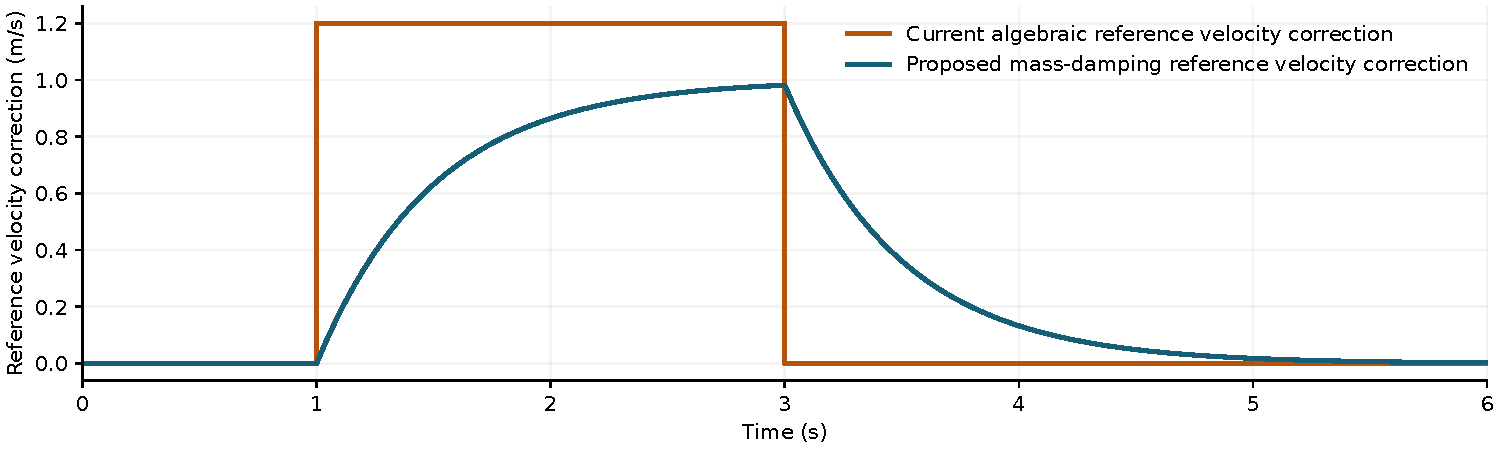
\includegraphics[width=\linewidth]{figures/reference_dynamics.pdf}
\caption{旧版 H6 基线与无力阈值、无状态清零的理想质量--阻尼模型。$1\le t<3\,\mathrm s$ 时施加 $20\,\mathrm N$ 正拉，其余时间为零。曲线均为参考量的计算结果。}
\end{figure}

后续可在统一参考和相同数据预算下，对比速度策略的监督模仿与 PPO，并比较直接测力、本体观测监督估计及循环网络估计。完整关节级 teacher--student 与冻结底座方案分别报告结果。
